\documentclass[11pt]{standalone}
\usepackage{amssymb}
\usepackage{amsmath}
\usepackage[no-math]{fontspec}
\usepackage{unicode-math}
\usepackage{libertinus}
\usepackage{pgf,xcolor}
\usepackage{tikz}
\usetikzlibrary{arrows.meta, backgrounds}
\usepackage{pgfplots}
\pgfplotsset{compat=newest}

\definecolor{my_darkgray}{HTML}{484949}
\definecolor{my_lightgray}{HTML}{F3F4F4}
\definecolor{my_darkblue}{HTML}{005A94}
\definecolor{my_lightblue}{HTML}{CCDEE9}
\definecolor{my_yellow}{HTML}{FFEC7F}
\definecolor{my_red}{HTML}{E60000}
\definecolor{my_orange}{HTML}{E87846}

\begin{document}
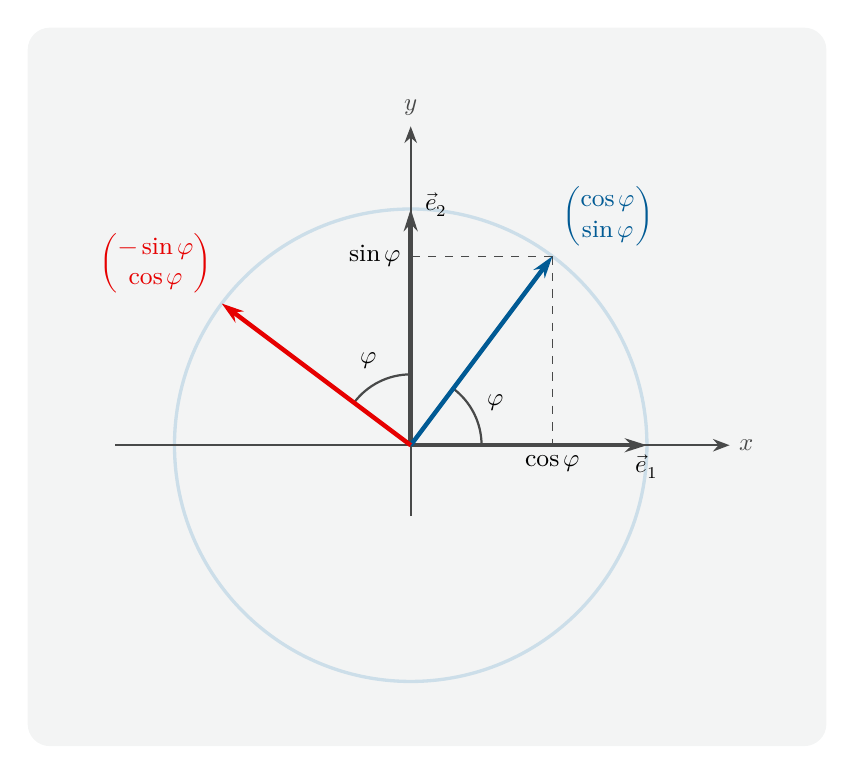
\begin{tikzpicture}[
    show background rectangle,
    background rectangle/.style={fill=my_lightgray, rounded corners=8pt},
    inner frame sep=0.8cm,
    x=3cm, y=3cm,
    vec/.style={-{Stealth[length=8pt, width=5pt]}, ultra thick},
    hilfe/.style={my_darkgray, dashed}
]

% ---------------------------------------------------------------
%  Drehung um phi = arccos(3/5), ca. 53.13 Grad (Matrix A aus 5.2)
%    D e1 = (cos phi, sin phi) = (0.6, 0.8)
%    D e2 = (-sin phi, cos phi) = (-0.8, 0.6)
% ---------------------------------------------------------------

% Einheitskreis
\draw[my_lightblue, very thick] (0, 0) circle (1);

% Achsen
\draw[-{Stealth[length=6pt]}, thick, my_darkgray] (-1.25, 0) -- (1.35, 0)
    node[right, font=\small] {$x$};
\draw[-{Stealth[length=6pt]}, thick, my_darkgray] (0, -0.3) -- (0, 1.35)
    node[above, font=\small] {$y$};

% Hilfslinien zu cos phi und sin phi
\draw[hilfe] (0.6, 0.8) -- (0.6, 0);
\draw[hilfe] (0.6, 0.8) -- (0, 0.8);
\node[below, font=\small] at (0.6, 0) {$\cos\varphi$};
\node[left, font=\small] at (0, 0.8) {$\sin\varphi$};

% Winkelboegen
\draw[my_darkgray, thick] (0.3, 0) arc (0:53.13:0.3);
\node[font=\small] at (26.6:0.4) {$\varphi$};
\draw[my_darkgray, thick] (0, 0.3) arc (90:143.13:0.3);
\node[font=\small] at (116.6:0.4) {$\varphi$};

% Einheitsvektoren
\draw[vec, my_darkgray] (0, 0) -- (1, 0);
\node[below, font=\small] at (1, 0) {$\vec{e}_1$};
\draw[vec, my_darkgray] (0, 0) -- (0, 1);
\node[right, font=\small] at (0.02, 1.02) {$\vec{e}_2$};

% Bilder der Einheitsvektoren
\draw[vec, my_darkblue] (0, 0) -- (0.6, 0.8);
\node[above right, font=\small, my_darkblue] at (0.6, 0.8)
    {$\begin{pmatrix} \cos\varphi \\ \sin\varphi \end{pmatrix}$};
\draw[vec, my_red] (0, 0) -- (-0.8, 0.6);
\node[above left, font=\small, my_red] at (-0.8, 0.6)
    {$\begin{pmatrix} -\sin\varphi \\ \cos\varphi \end{pmatrix}$};

\end{tikzpicture}
\end{document}
